\subsubsection{Combustor [Cameron Ellis]}

The combustor consisted of a rotating detonation engine surrounded by an inner and outer wall that were each coated in TBC and regeneratively cooled. Heat transfer through the walls was calculated using a modified form of Bartz equation in order to calculate the heat transfer coefficient hg inside the combustor. Equation \ref{eqn:modBartz} shows the standard form of Bartz equation for a rocket nozzle.

\begin{equation}
h_g = \left[ \frac{0.026}{D_t^{0.2}}\left(\frac{\mu^{0.2}C_p}{Pr^{0.6}}\right)_{ns} \left( \frac{(p_c)_{ns}g}{c^*} \right)^{0.8} \left(\frac{D_t}{R}\right)^{0.1} \right] \left(\frac{A_t}{A}\right)^{0.9}\sigma
\label{eqn:modBartz}
\end{equation}

Where the $ns$ subscript denotes values of the gas inside of the combustor, and where sigma is the correction factor denoted by Equation \ref{eqn:longSigma}.

\begin{equation}
\sigma=\frac{1}{\left[ \frac{1}{2} \frac{T_{wg}}{(T_c)_{ns}} \left( 1 + \frac{\gamma - 1}{2}M^2\right)+\frac{1}{2}\right]^{0.68} \left[1+\frac{\gamma-1}{2}M^2\right]^{0.12}}
\label{eqn:longSigma}
\end{equation}

For this combustor, there is no nozzle radius of curvature, denoted by R in the Bartz equation, so the term $\left(\frac{D_t}{R}\right)^{0.1}$ becomes 1. Furthermore, the area of the throat and the area of the combustor are equal since they have the same radius, so the area ratio term $\left(\frac{A_t}{A}\right)^{0.9}$ also becomes 1. Once an $hg$ value was obtained, a guess at the hot side wall temperature, $T_{wg}$ was taken and used to calculate heat flux from the combustor to the surface of the wall. This heat flux was then compared to the heat flux from the liquid coolant to the cold side of the wall, and compared together. The hot side wall temperature then changed iteratively until the two heat flux values matched. This was done across the entire length of the combustor, and was used to find the temperatures of the TBC inside the combustor, the temperature of the metal inside combustor wall, and the temperature of the ethylene in order to make sure boiling would not occur.

\begin{wrapfigure}{r}{0.6\textwidth}
\begin{center}
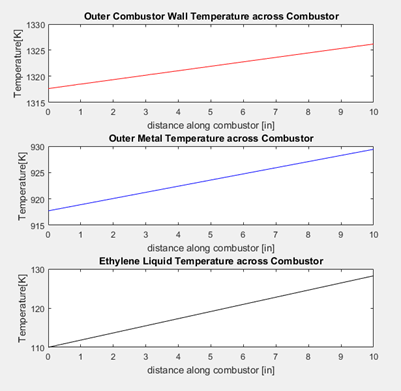
\includegraphics[width=0.6\textwidth]{combustorWallTemps}
\caption{Temperature Range Across Combustor Structure}
\label{fig:combustorWallTemps}
\end{center}
\end{wrapfigure}

Figure \ref{fig:combustorWallTemps} shows the temperature of the TBC, inside metal wall, and the ethylene across the length of the combustor. The TBC experiences temperatures of upwards of 1327 K at the hottest points after regenerative cooling is applied. The metal wall experiences up to 930 K, and therefore a material that could withstand those temperatures without going past its deformation temperature had to be selected. Incoloy 800 HT was chosen due to its high heat resistance. At the calculated temperatures, the alloy would be able to work at about 60\% of its intended strength. The TBC coating selected was NAS3-23944, a super TBC created by NASA.

Figure \ref{fig:incoloyPlot} displays the elongation, tensile strength, and yield strength for INCOLOY 800HT for various temperatures. Though at the temperatures the RDE combustor would be operating at would affect the strength of the INCOLOY, it is still within a reasonable operating range for the metal work as intended.

To regeneratively cool both sides of the combustor, the mass flow rate of the liquid ethylene had to be split up between the inner and outer walls. Since the inner wall has a lower surface area, it would need less cooling channels, while the larger outer wall would need more. The cooling channels were split into 100 channels on the inner wall and 120 channels on the outer wall. Each cooling channel has a dimension of 0.215”x0.125” The mass split of the fuel ended up being 48.5\% of fuel going to the inner regenerative cooling, and 51.5\% of fuel going towards the outer regenerative cooling.  This allows the two walls to experience approximately the same heat transfer, so the same thickness of thermal barrier coating would be able to be used on both sides. This was done to ensure that one side would not need to thick a layer of thermal barrier coating and increase the chance of cracking and flaking to take place during combustion.

